\documentclass[12pt]{article}
\usepackage[a4paper,margin=2.5cm]{geometry}
\usepackage{amsmath, amssymb, amsthm}
\usepackage{bm}
\usepackage{hyperref}
\usepackage{graphicx}
\usepackage{caption}
\usepackage{listings}
\usepackage{xcolor}
\usepackage{float}
\usepackage{placeins}
\graphicspath{{figures/}}

% Code style
\lstdefinestyle{code}{
  basicstyle=\ttfamily\small,
  numbers=left,
  numberstyle=\tiny,
  numbersep=8pt,
  keywordstyle=\color{blue},
  commentstyle=\color{teal!70!black},
  stringstyle=\color{orange!70!black},
  showstringspaces=false,
  breaklines=true,
  frame=single,
  framerule=0.3pt,
  rulecolor=\color{black!15}
}
\lstset{style=code}

\title{Attention Mechanisms and Transformers}
\author{}
\date{\today}

\begin{document}
\maketitle

\section{Motivation and Formulation of Attention}
Attention mechanisms allow models to focus on relevant parts of the input when producing outputs. Given queries $\mathbf{Q}$, keys $\mathbf{K}$, and values $\mathbf{V}$, the additive attention score between a query $\mathbf{q}_i$ and key $\mathbf{k}_j$ is
\begin{equation}
  e_{ij} = \mathbf{v}^{\top} \tanh(\mathbf{W}_q \mathbf{q}_i + \mathbf{W}_k \mathbf{k}_j),
\end{equation}
while scaled dot-product attention simplifies the score to
\begin{equation}
  \mathrm{Attention}(\mathbf{Q}, \mathbf{K}, \mathbf{V}) = \mathrm{softmax}\left( \frac{\mathbf{Q} \mathbf{K}^{\top}}{\sqrt{d_k}} \right) \mathbf{V}.
\end{equation}
The softmax weights act as adaptive alignment coefficients. Figure~\ref{fig:attention_scores} illustrates how attention redistributes focus across sequence elements.

\subsection{Alignment and Context Vectors}
For sequence-to-sequence tasks, attention forms context vectors $\mathbf{c}_i = \sum_j \alpha_{ij} \mathbf{v}_j$ with $\alpha_{ij}$ from the softmax weights. Attention improves convergence, mitigates information bottlenecks, and handles variable-length inputs.

\subsection{Variations}
Common variants include additive (Bahdanau) attention, multiplicative (Luong) attention, and location-based attention. Monotonic attention enforces ordered alignments for speech recognition. Sparse and hard attention restrict selections to top-$k$ elements for efficiency.

\section{Self-Attention and Multi-Head Attention}
Self-attention treats the same sequence as queries, keys, and values, enabling long-range dependencies without recurrence. Multi-head attention (MHA) projects inputs into $h$ subspaces and attends in parallel:
\begin{align}
  \mathrm{head}_i &= \mathrm{Attention}(\mathbf{Q} \mathbf{W}_i^Q, \mathbf{K} \mathbf{W}_i^K, \mathbf{V} \mathbf{W}_i^V), \\
  \mathrm{MHA}(\mathbf{Q}, \mathbf{K}, \mathbf{V}) &= \mathrm{Concat}(\mathrm{head}_1, \ldots, \mathrm{head}_h) \mathbf{W}^O.
\end{align}
Multi-heads capture diverse relational patterns (e.g., syntax, positional cues). Figure~\ref{fig:self_attention_heads} visualizes head-specific attention maps.

\subsection{Positional Encoding}
Because self-attention is permutation-invariant, transformers add positional encodings. Sinusoidal encodings use fixed frequencies:
\begin{align}
  \mathrm{PE}_{(pos, 2i)} &= \sin\left( \frac{pos}{10000^{2i/d_{\text{model}}}} \right), \\
  \mathrm{PE}_{(pos, 2i+1)} &= \cos\left( \frac{pos}{10000^{2i/d_{\text{model}}}} \right).
\end{align}
Learned positional embeddings or rotary positional embeddings (RoPE) adapt positions during training and improve extrapolation.

\subsection{Efficiency Considerations}
Self-attention has $\mathcal{O}(n^2)$ complexity. Sparse, local, or linear attention variants (e.g., Performer, Linformer) reduce cost for long sequences by approximating attention weights or restricting receptive fields.

\section{Transformer Architecture}
The transformer encoder-decoder architecture comprises stacked layers with MHA and feed-forward networks (FFNs). Each encoder layer performs:
\begin{align}
  \mathbf{z} &= \mathrm{LayerNorm}(\mathbf{x} + \mathrm{MHA}(\mathbf{x})), \\
  \mathbf{y} &= \mathrm{LayerNorm}(\mathbf{z} + \mathrm{FFN}(\mathbf{z})),
\end{align}
where FFN is typically a two-layer MLP with ReLU or GELU activation. Decoder layers include masked self-attention and cross-attention to the encoder outputs. Residual connections and layer normalization stabilize deep stacks.

\subsection{Feed-Forward Networks}
The position-wise FFN expands dimensionality (e.g., $d_{\text{model}}=512$ to $2048$) before projecting back. Variants like gated linear units (GLU), SwiGLU, or depthwise convolutions enhance expressive power. Dropout and stochastic depth regularize training.

\subsection{Training Strategies}
Transformers rely on large-scale data and parallel computation. Techniques include label smoothing, warmup schedules, adaptive optimizers (Adam, Adafactor), gradient accumulation, and mixed-precision training.

\begin{figure}[H]
  \centering
  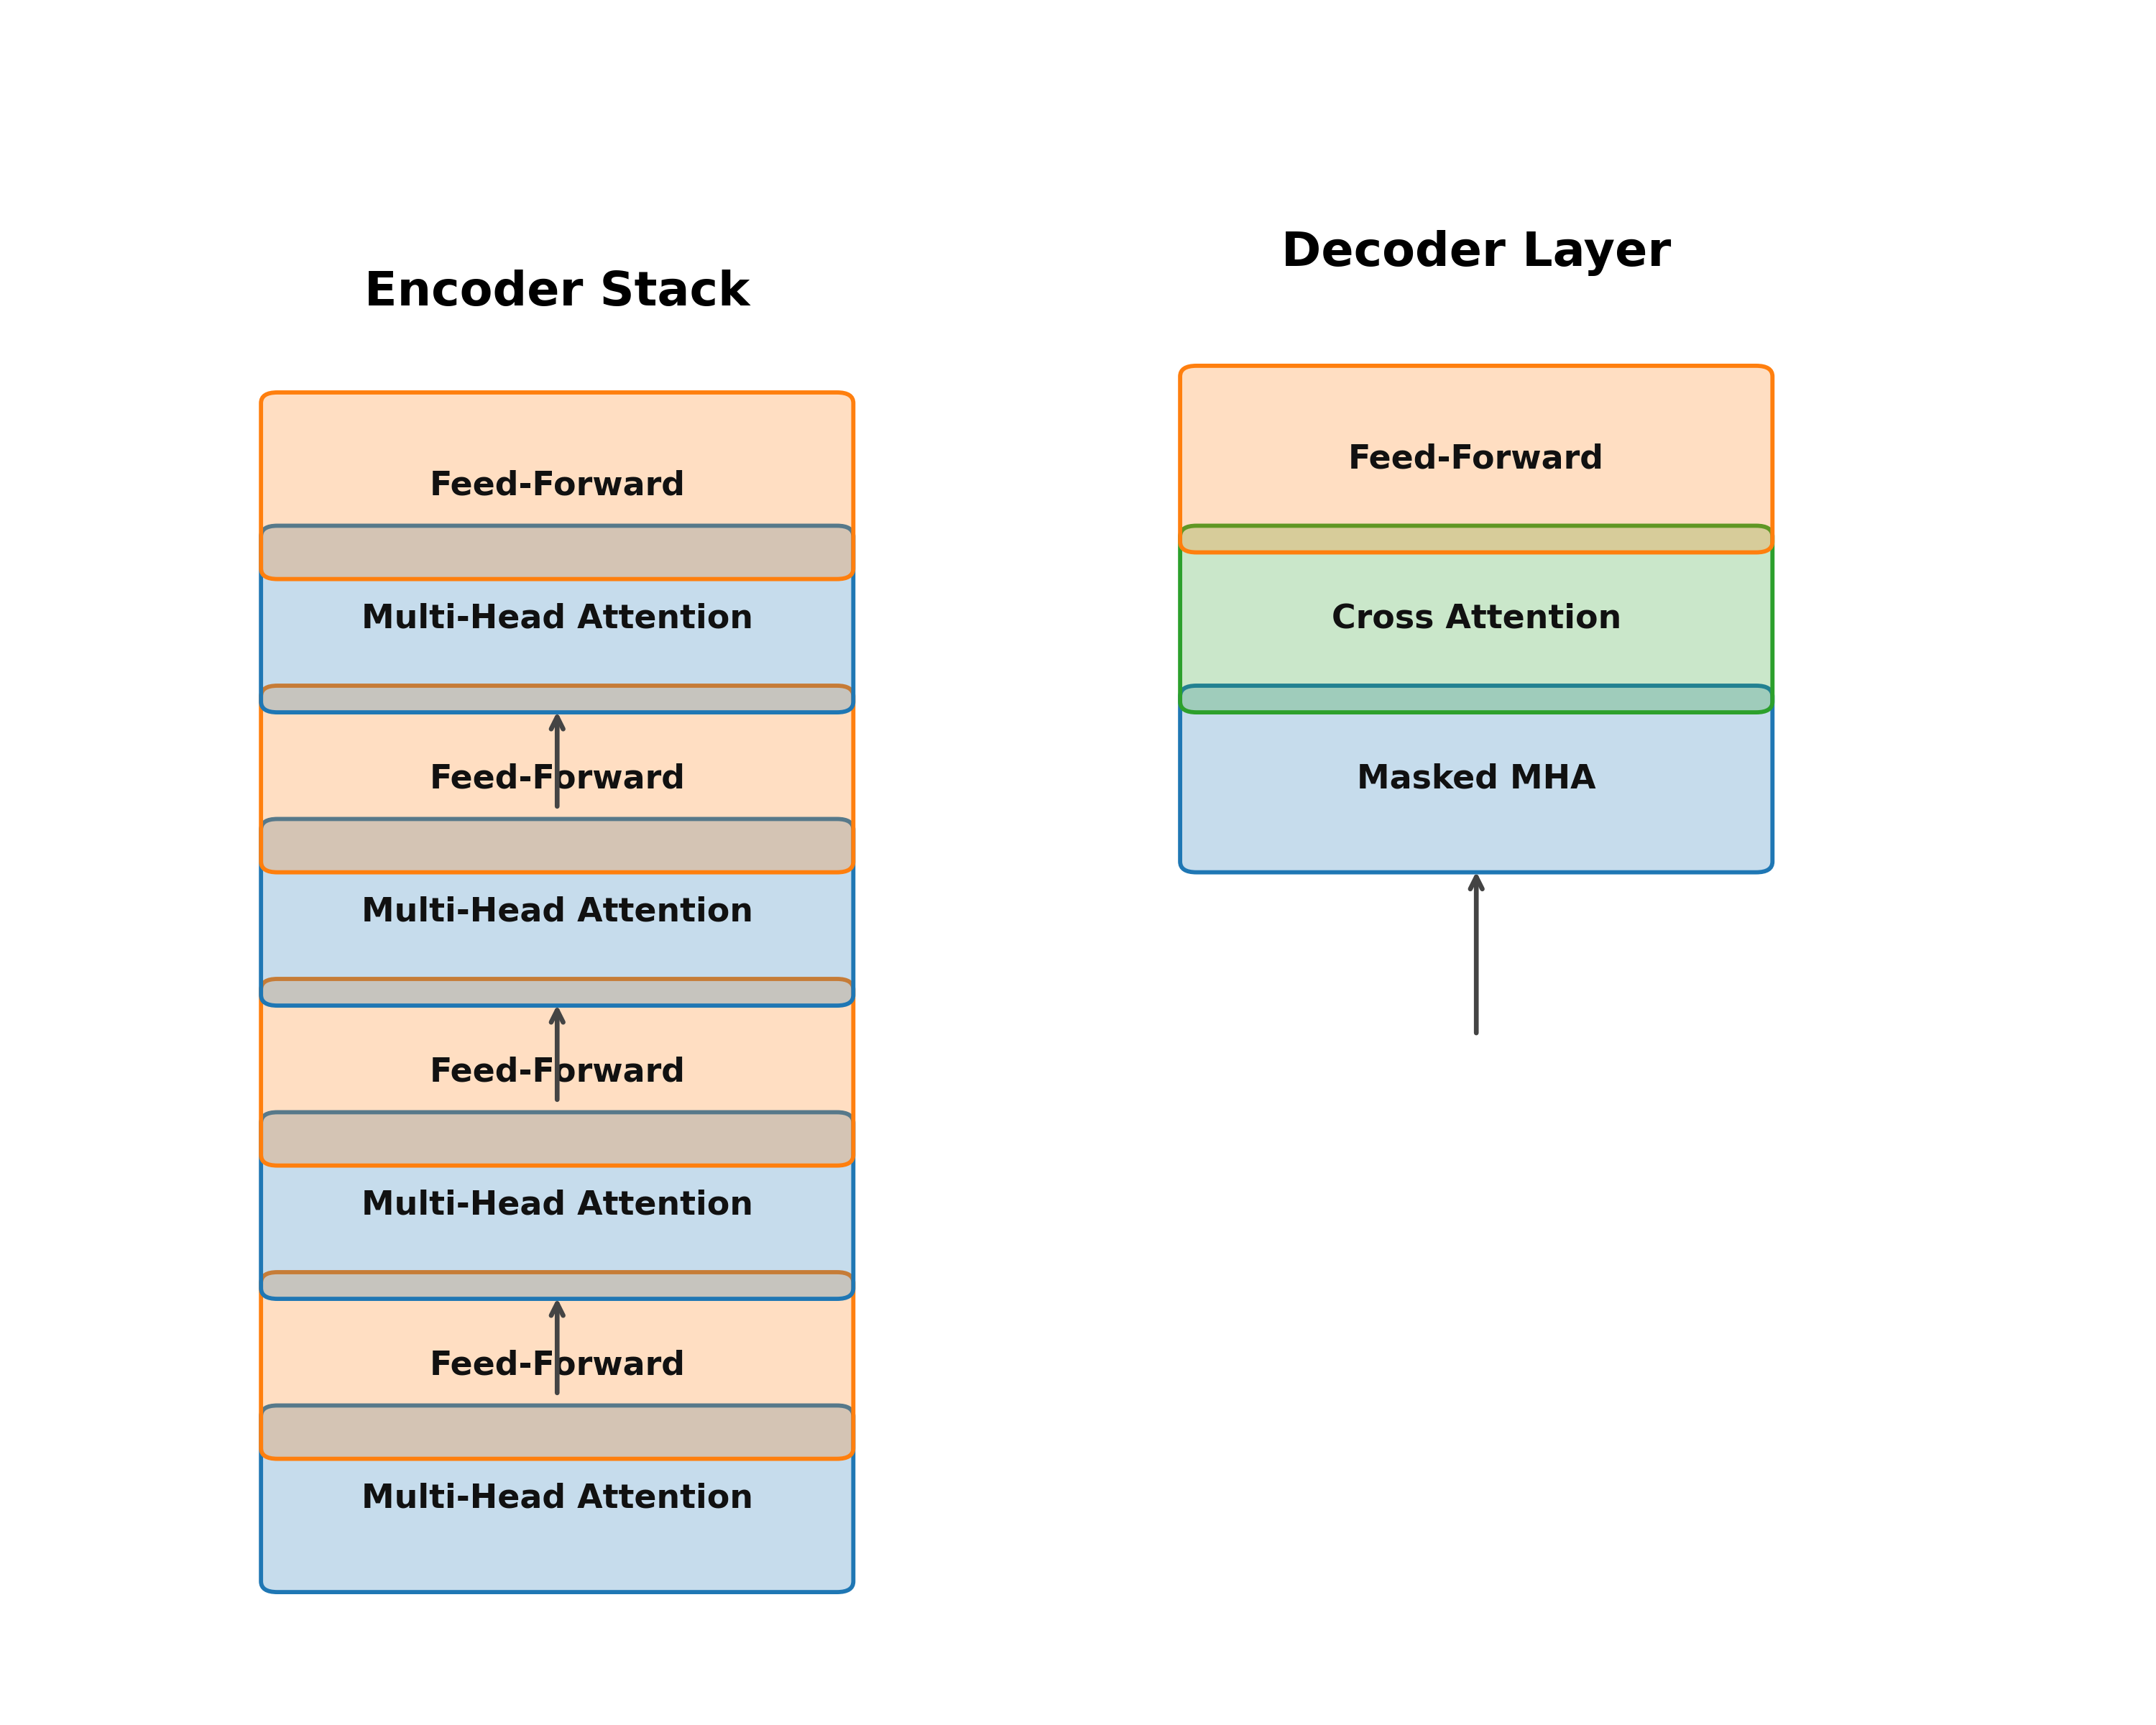
\includegraphics[width=0.85\linewidth]{transformer_layer_stack.png}
  \caption{Transformer encoder-decoder stack with self-attention, cross-attention, and position-wise feed-forward networks.}
  \label{fig:transformer_stack}
\end{figure}
\FloatBarrier

\section{Pretrained Language Models: BERT and GPT}
Pretrained transformers revolutionized NLP by learning contextual representations.

\subsection{BERT}
Bidirectional Encoder Representations from Transformers (BERT) pretrains using masked language modeling (MLM) and next sentence prediction (NSP). The model uses only the encoder stack with bidirectional self-attention, enabling deep contextual understanding. Fine-tuning BERT for downstream tasks requires minimal adaptation (task-specific heads atop [CLS]).

\subsection{GPT Series}
Generative Pretrained Transformers (GPT) employ decoder-only architectures trained with causal language modeling. Autoregressive training predicts the next token given past context. Scaling laws reveal predictable improvements with larger models and data. GPT-2/3 introduced zero-shot and few-shot prompting; GPT-4 incorporated multi-modal inputs and tool integration.

\subsection{Comparison and Extensions}
BERT excels at understanding tasks (classification, QA), whereas GPT excels at generation. Hybrid models (T5, BART) unify encoder-decoder training objectives. Instruction tuning, reinforcement learning from human feedback (RLHF), and retrieval augmentation further enhance performance.

\section{Applications in NLP and Cross-Modal Learning}
Attention and transformers underpin modern AI systems.

\subsection{Natural Language Processing}
Transformers dominate machine translation, summarization, sentiment analysis, and question answering. Pretrained encoders provide embeddings for information retrieval; sequence-to-sequence transformers power neural machine translation and abstractive summarization.

\subsection{Cross-Modal and Multimodal Learning}
Vision transformers (ViT) apply self-attention to image patches. CLIP aligns text and images via contrastive pretraining. Video transformers model spatio-temporal dependencies. Audio transformers handle speech recognition and music generation. Multimodal large language models integrate vision, text, and audio for grounded reasoning.

\subsection{Knowledge Integration}
Retrieval-augmented models (RAG), memory-augmented transformers, and adapters incorporate external knowledge bases. Prompt tuning and LoRA (low-rank adaptation) provide parameter-efficient fine-tuning.

\begin{figure}[H]
  \centering
  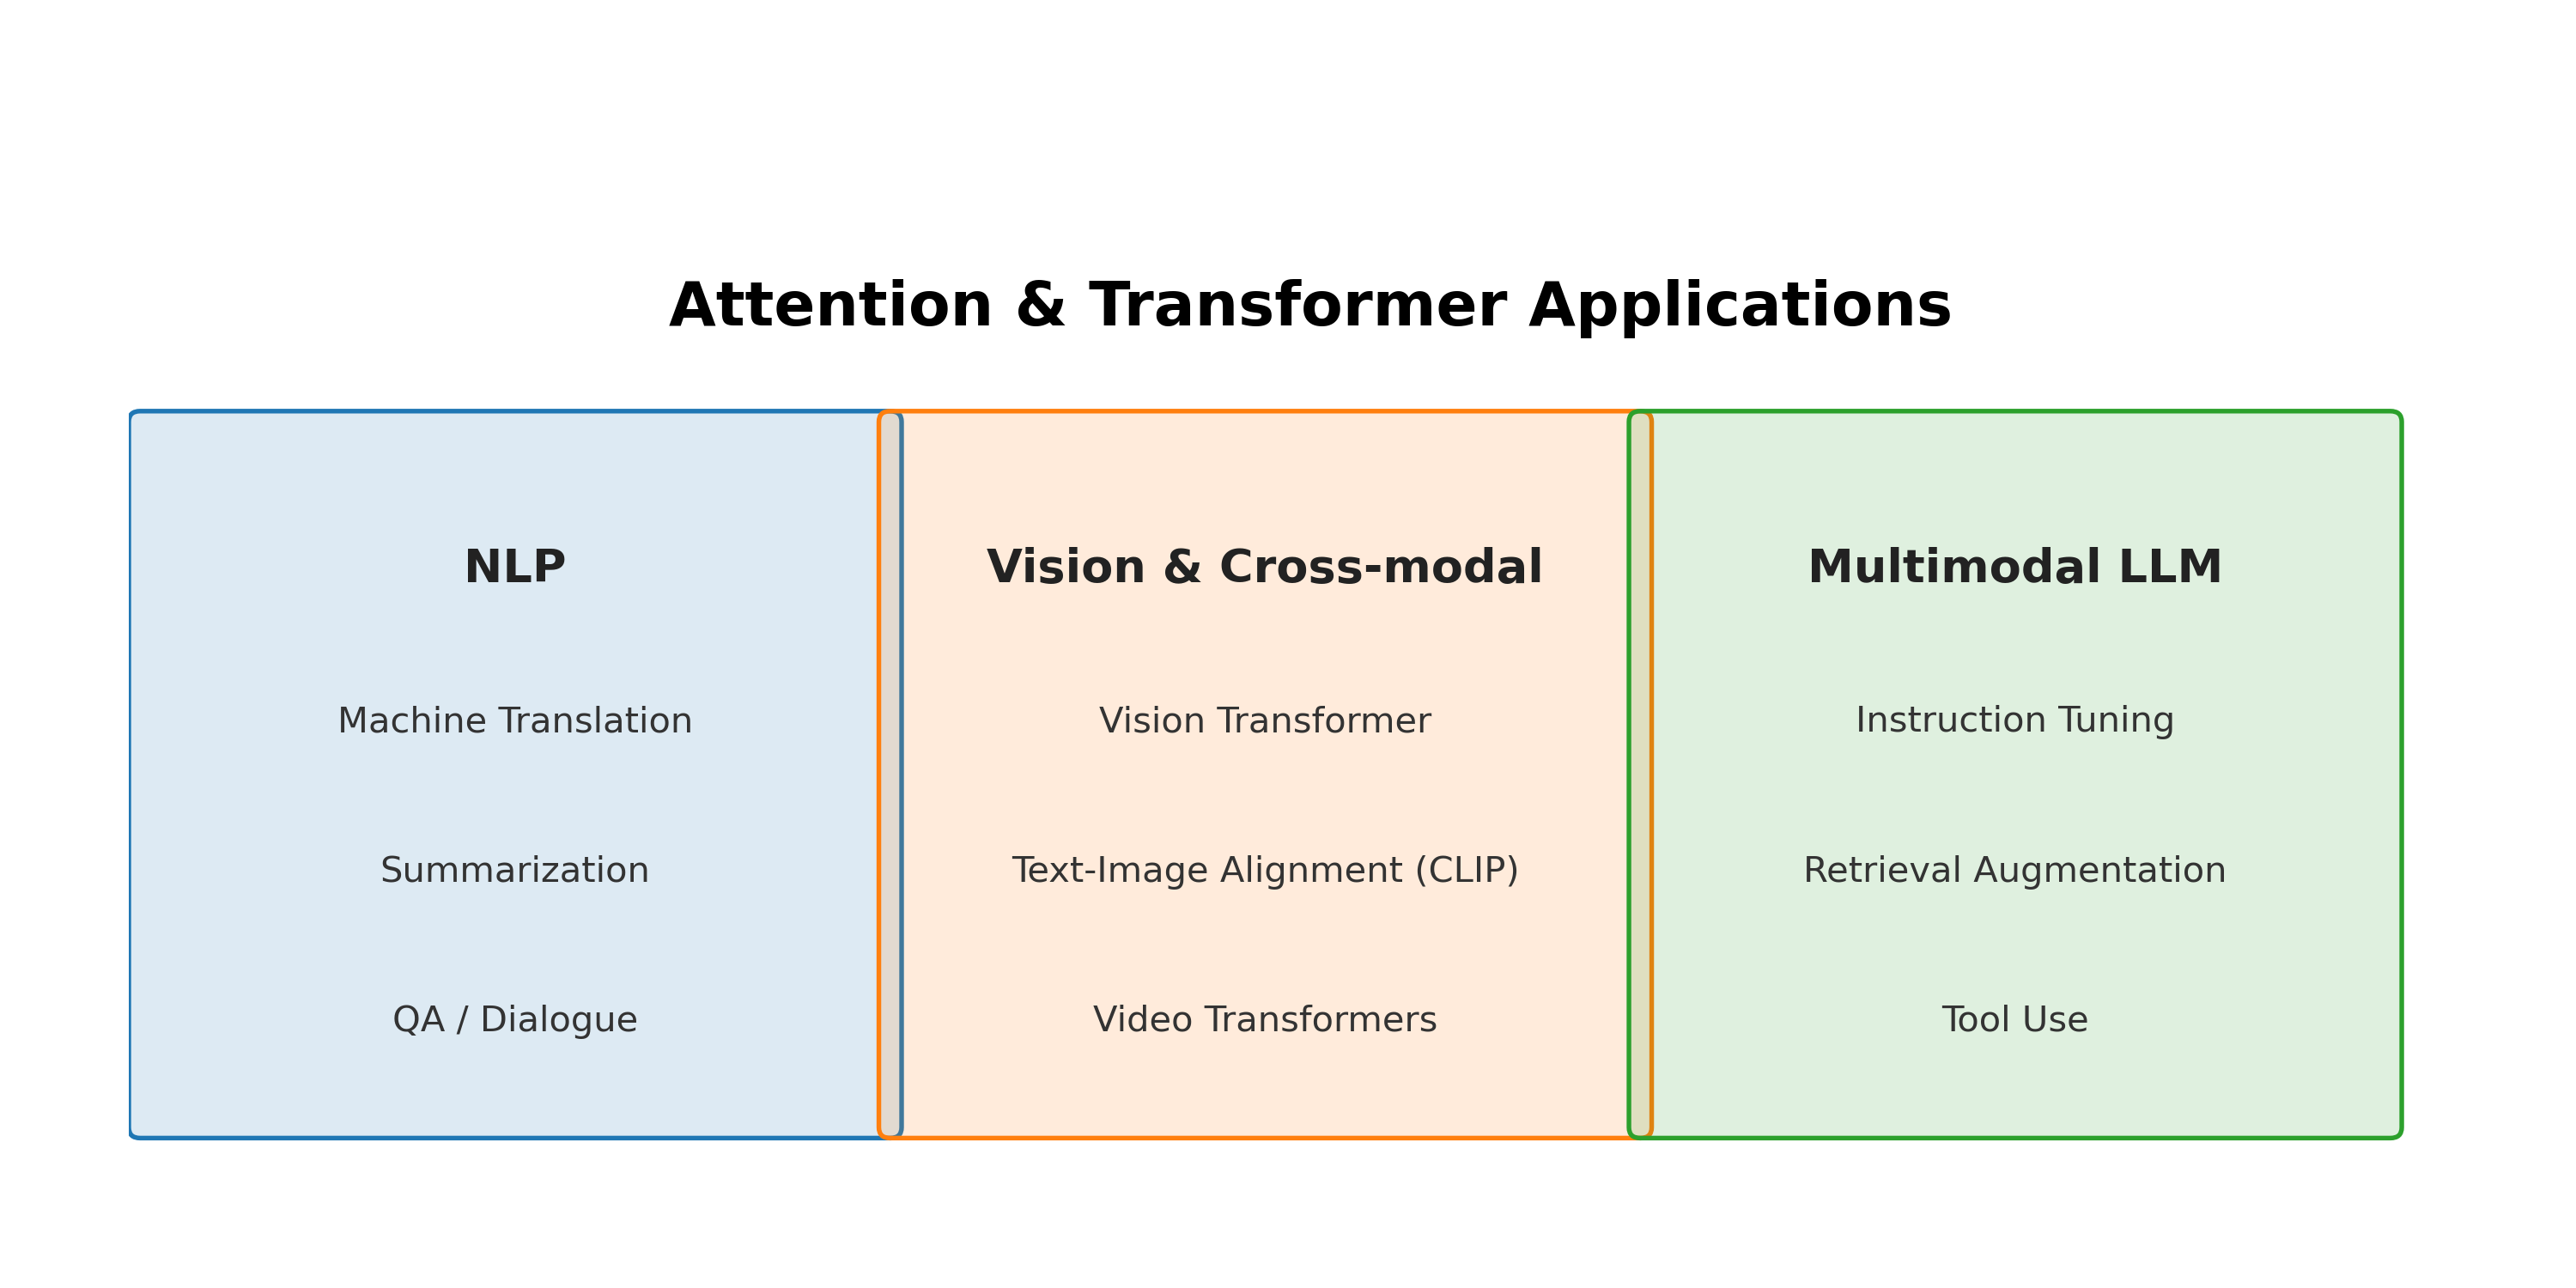
\includegraphics[width=0.85\linewidth]{attention_transformer_applications.png}
  \caption{Applications of attention and transformers in NLP and multimodal settings.}
  \label{fig:transformer_applications}
\end{figure}
\FloatBarrier

\section{Practical Tips}
\begin{itemize}
  \item \textbf{Memory management:} Use gradient checkpointing, mixed precision, or sequence chunking to handle long sequences.\item \textbf{Regularization:} Apply dropout, attention dropout, label smoothing, and weight decay to prevent overfitting.\item \textbf{Scaling:} Monitor loss scaling laws; adjust batch size, learning rate schedule (cosine with warmup), and gradient clipping.\item \textbf{Evaluation:} Track task-specific metrics (BLEU, ROUGE, accuracy) and perplexity. Analyze attention maps and calibration.\item \textbf{Deployment:} Distill large models into smaller students, quantize weights, or apply sparse attention for latency-sensitive applications.\end{itemize}

\end{document}
